\documentclass{beamer}

\mode<presentation>
{
  \usetheme{Antibes}
  \usecolortheme{beaver}
  % or ...

  \setbeamercovered{transparent}
  % or whatever (possibly just delete it)
}


\usepackage[english]{babel}
\usepackage[utf8]{inputenc}
\usepackage{times}
\usepackage[T1]{fontenc}
\usepackage{graphicx}
\usepackage[compatibility=false]{caption}
\usepackage{subcaption}
\usepackage{physics}
\usepackage{amsmath}
\usepackage{amssymb}

%\usepackage{multimedia}
%\usepackage{movie9}


\newcommand{\expv}[1]{\ensuremath{\mathbb{E}[ #1]}}
\newcommand{\xs}[2]{\ensuremath{\Sigma_{#1}^{(#2)}}}
\newcommand{\intO}{\ensuremath{\int\limits_{4\pi}}}
\newcommand{\intz}{\ensuremath{\int\limits_0^1}}
\newcommand{\intf}{\ensuremath{\int\limits_{-\infty}^\infty}}
\newcommand{\intzf}{\ensuremath{\int\limits_{0}^\infty}}

\title[Multistep Input Reduction]
{Multistep Input Reduction for High Dimensional Uncertainty Quantification}

%\subtitle
%{A Term Project}

\author[Talbot] % (optional, use only with lots of authors)
{Paul W. Talbot\inst{1}, CongJian Wang\inst{2}, \\ Cristian Rabiti\inst{2}, Anil K. Prinja\inst{1}}


\institute[University of New Mexico] % (optional, but mostly needed)
{
  \inst{1}%
  University of New Mexico\\
  \inst{2}
  Idaho National Laboratory
}

\date[PHYSOR 2016] % (optional, should be abbreviation of conference name)
{PHYSOR 2016, Sun Valley, Idaho}


\subject{Multistep Uncertainty Quantification}

\pgfdeclareimage[height=0.75cm]{university-logo}{graphics/INL}
\logo{\pgfuseimage{university-logo}}

\addtobeamertemplate{navigation symbols}{}{
  \usebeamerfont{footline}%
  \usebeamercolor[fg]{footline}%
  \hspace{1em}%
  \insertframenumber/\inserttotalframenumber
}

\begin{document}

\begin{frame}
  \titlepage
\end{frame}

\begin{frame}{Outline}{Discussion Points}\vspace{-20pt}
  \tableofcontents%[pausesections]
  % You might wish to add the option [pausesections]
\end{frame}

%                                                  %
%                 INTRODUCTION                     %
%                                                  %
\section{Introduction}
% UQ is useful in reactor physics
\begin{frame}{Introduction}{Uncertainty Quantification}\vspace{-30pt}
  %benefits, uses of UQ
  How well do we know what we know?
  \vspace{10pt}
  \begin{itemize}
    \item Quantity of Interest Distribution
    \item Failure Probabilities
    \item Accurate Margins
  \end{itemize}
\end{frame}
% UQ methods: MC and Collocation, pros and cons
\begin{frame}{Introduction}{Uncertainty Quantification Methods}\vspace{-30pt}
  Monte Carlo, Latin Hypercube
  \begin{itemize}
    \item (Mostly) Agnostic of Dimensionality
    \item Very slow in converging $\left(\frac{c}{\sqrt{N}}\right)$
  \end{itemize}
  \vspace{15pt}
  Grid-based Polynomial Expansions
  \begin{itemize}
    \item Fast convergence for low (<50) dimensions
    \item Very slow convergence for high (>1000) dimensions
  \end{itemize}
\end{frame}
% Reactor physics problems are intrinsically high-dimensional
\begin{frame}{Introduction}{Uncertainty Quantification in Reactor Physics}\vspace{-30pt}
  Specific to Reactor Physics
  \begin{itemize}
    \item Large input spaces (tens of thousands)
    \item Computationally-intensive models
    \item Long solve times
  \end{itemize}
  \vspace{15pt}
  Want few samples to characterize high-dimensional input space
\end{frame}
% Reactor physics input spaces tend to be highly correlated
\begin{frame}{Introduction}{Uncertainty Quantification in Reactor Physics}\vspace{-30pt}
  Nature of input space
  \begin{itemize}
    \item Mostly cross sections
    \item Significant correlation between tabulation points, energies\dots
    \item Many cross sections have relatively low impact
  \end{itemize}
  \vspace{15pt}
  We can leverage these properties
\end{frame}
% Need to reduce size of input space for most efficiency
% Two approaches: input-input correlation, input-output correlation


%                                                  %
%                   METHODS                        %
%                                                  %
\section{Methods}
\subsection{PCA}
% PCA
\begin{frame}{Methods}{Principle Component Analysis}%\vspace{-30pt}
  Correlated input variables orthogonalized
  \begin{itemize}
    \item Start with many correlated ``manifest'' input dimensions
    \item Use linear PCA to pick characteristic ``latent'' dimensions
    \item Eliminate dimensions with sufficiently small impact
  \end{itemize}
  \vspace{5pt}
  \begin{equation}
    M \approx Q L \nonumber
  \end{equation}
  \vspace{-5pt}
  \begin{itemize}
    \item $M$ is the manifest set of input variables ($Nx1$),
    \item $Q$ is the PCA reduction matrix ($NxM$),
    \item $L$ is the reduced latent variables($Mx1$)
    \item $M \leq N$
  \end{itemize}
\end{frame}

\begin{frame}{Methods}{Principle Component Analysis}%\vspace{-30pt}
  \begin{figure}[h!]
    \centering
      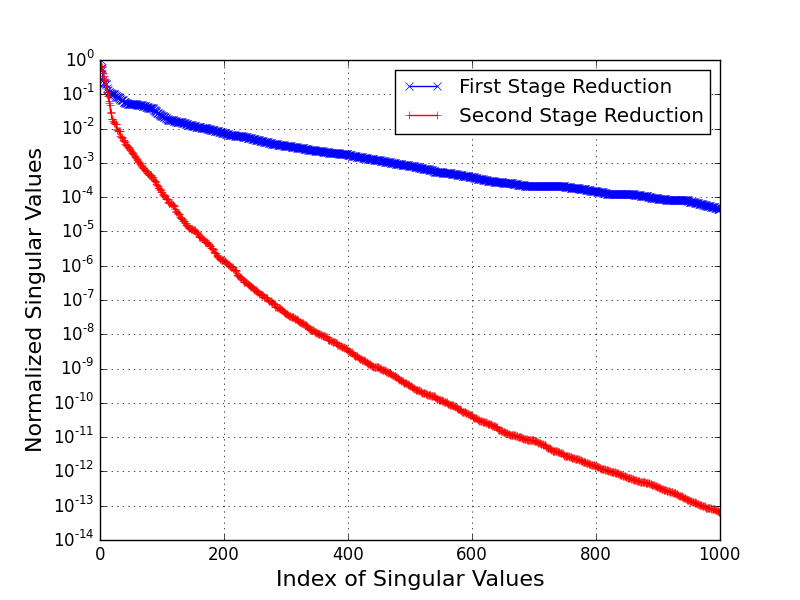
\includegraphics[width=0.7\textwidth]{graphics/PCA_1_2}
      \caption{PCA Reduction}
  \end{figure}
\end{frame}

% Sensitivity
\subsection{Sensitivity}
\begin{frame}{Methods}{Sensitivity-Based Reduction}%\vspace{-30pt}
  Eliminating low-impact inputs
  \begin{itemize}
    \item Calculate global sensitivity indices
    \item Remove inputs of low impact
  \end{itemize}
  \vspace{10pt}
  Calculation is often costly (Linear regression)
  %\vspace{10pt}
  \begin{equation}
    L \approx P R, \nonumber
  \end{equation}
  \begin{itemize}
    \item $L$ is the set of (once-reduced) input variables ($Mx1$),
    \item $P$ is the sensitivity reduction matrix ($MxK$),
    \item $R$ is the twice-reduced variables($Kx1$)
    \item $K \leq M$
  \end{itemize}
\end{frame}

\begin{frame}{Methods}{Sensitivity-Based Reduction}%\vspace{-30pt}
  \begin{figure}[h!]
    \centering
      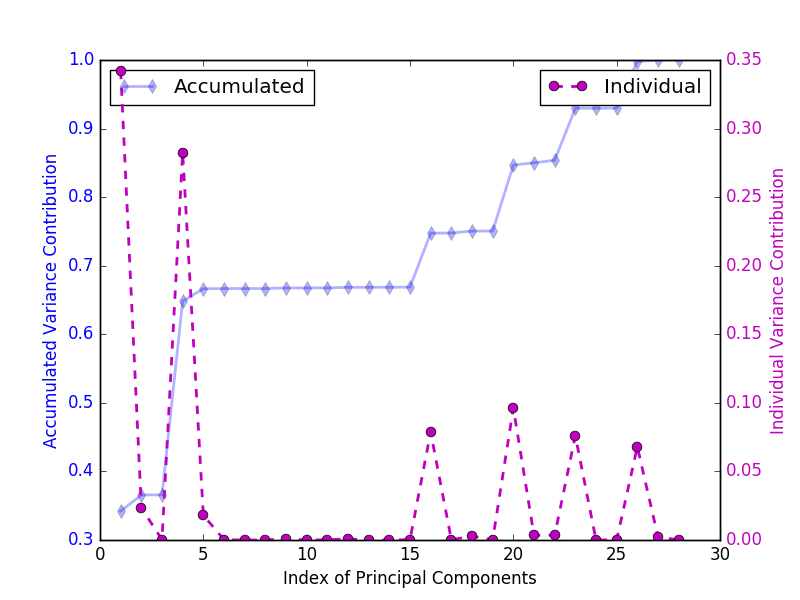
\includegraphics[width=0.7\textwidth]{graphics/variance_contribs_example.png}
      \caption{Sensitivity Reduction}
  \end{figure}
\end{frame}

% Together (work flow)
\begin{frame}{Methods}{Combined Reduction}%\vspace{-30pt}
  Combine PCA and Sensitivity Reduction
  \begin{equation}
    M \approx P Q R \nonumber
  \end{equation}
  \[|R| < |L| < |M|\]
  \vspace{10pt}
  Reduction can be several orders of magnitude
\end{frame}

%                                                  %
%                   RESULTS                        %
%                                                  %
\section{Results}
\begin{frame}{Results}{Demonstration Case}\vspace{-30pt}
  \begin{itemize}
    \item 308 correlated uncertain input variables
    \item Originally cross sections from SCALE 44-group library
    \item Manufactured for symmetric positive definite (not required)
  \end{itemize}
  Simulation is simple polynomial of input variables
\end{frame}

\begin{frame}{Results}{Demonstration Procedure}\vspace{-30pt}
  \begin{enumerate}
    \item Use Monte Carlo to establish benchmark ($N=308$)
    \item Perform PCA reduction TODO keep what? ($M=50$)
    \item Use Monte Carlo to sample PCA-reduced space ($M=50$)
    \item Perform Sensitivity Analysis
    \item Use Monte Carlo to sample various sensitivity reductions
  \end{enumerate}
\end{frame}

\begin{frame}{Results}{Demonstration: PCA Reduction}\vspace{-30pt}
  Leading Coefficients
  \begin{tabular}{c|c|c}
    Rank & Dimension & Coefficient \\ \hline
    1 & 1 & TODO
  \end{tabular}
\end{frame}

\begin{frame}{Results}{Demonstration Twice-Reduced Mean}\vspace{-30pt}
  \begin{figure}[h!]
    \centering
    \begin{subfigure}[b]{0.49\textwidth}
      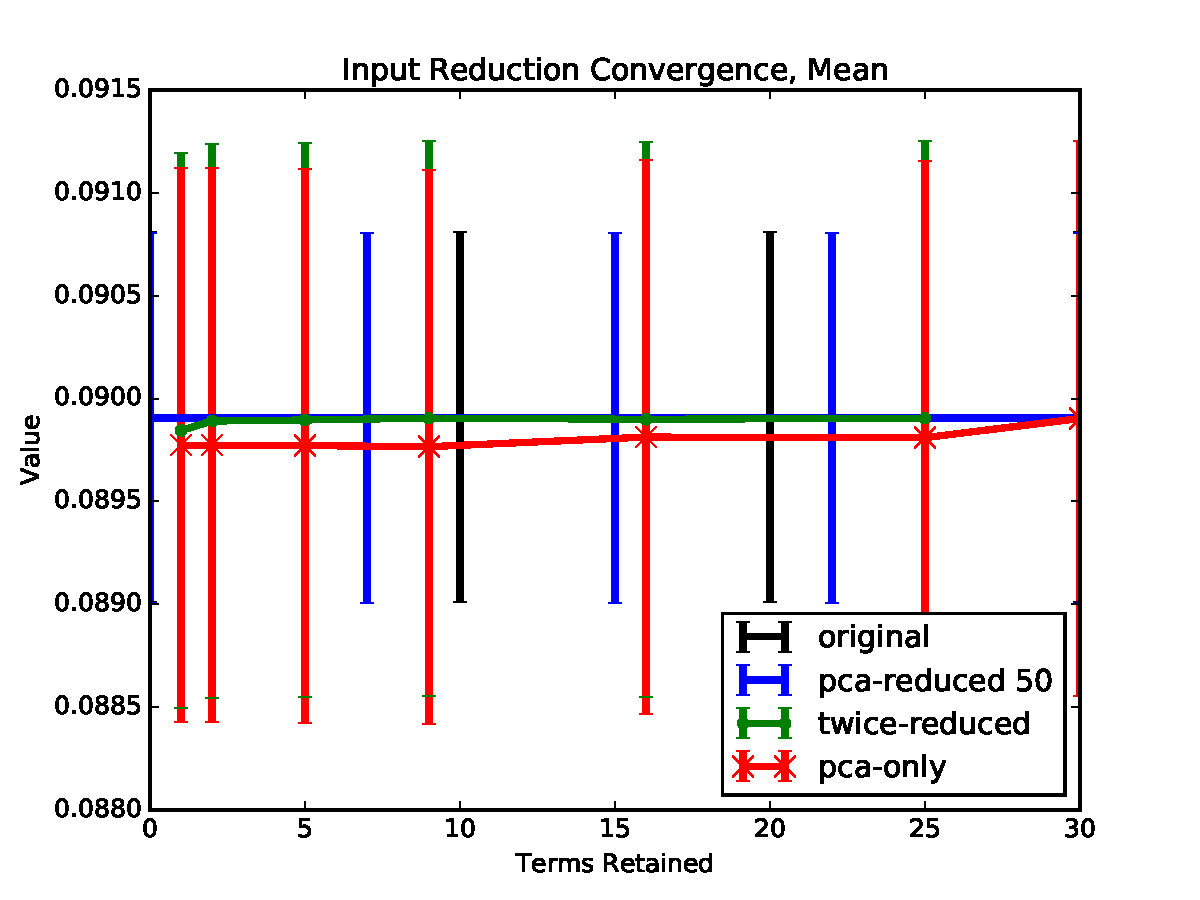
\includegraphics[width=\textwidth]{graphics/mean}
      \caption{Mean Values}
      \label{twice 9v mean val}
    \end{subfigure}
    \begin{subfigure}[b]{0.49\textwidth}
      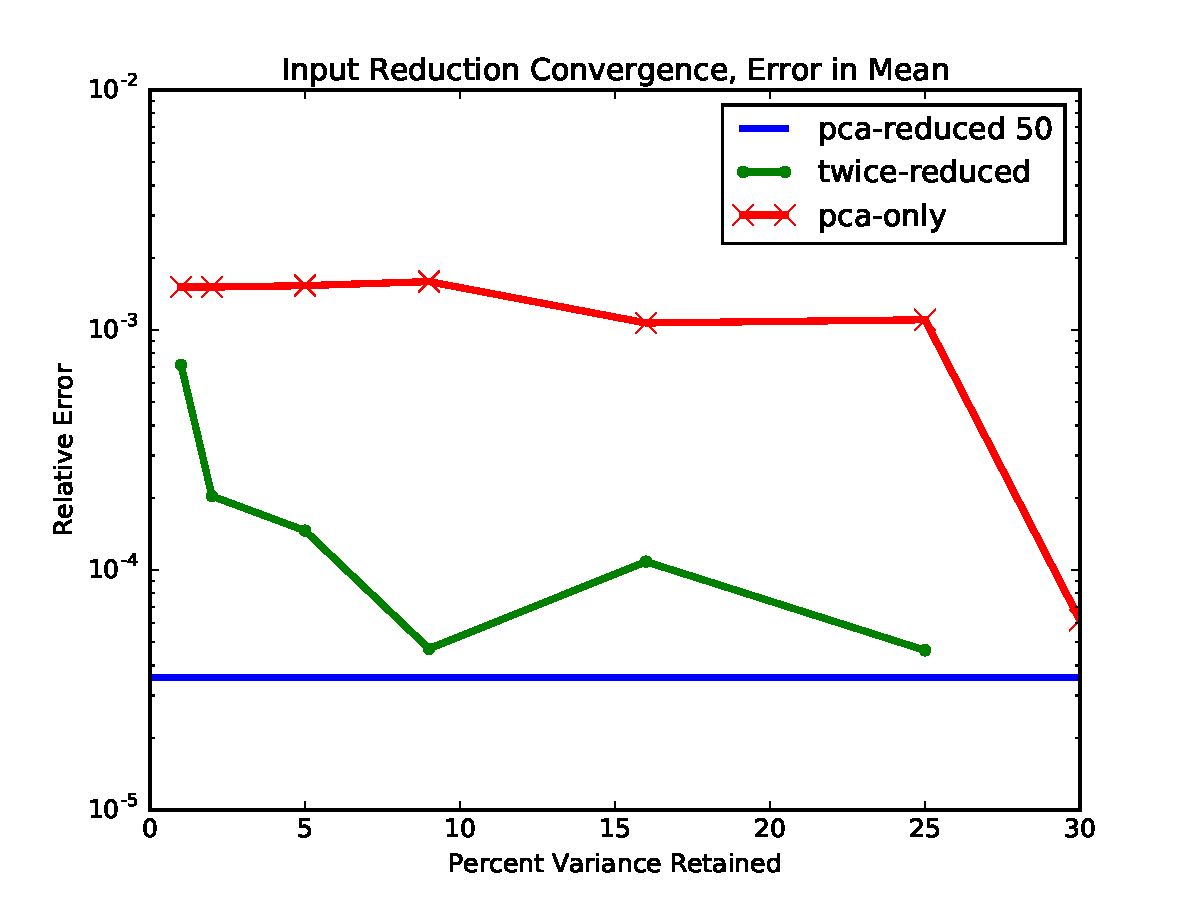
\includegraphics[width=\textwidth]{graphics/mean_err}
      \caption{Mean Errors}
      \label{twice 9v mean err}
    \end{subfigure}
  \end{figure}
\end{frame}

\begin{frame}{Results}{Demonstration Procedure}\vspace{-30pt}
  todo adaptive sobol bonus
\end{frame}
% Demonstration case: 308 variable model
%  - PCA reduction
%  - Sensitivity reduction
%  - Combined
%  - Adaptive Sobol: doing the sensitivity reduction for you
%  - Plots



\end{document}






\begin{frame}{Uncertainty Quantification}{Results: pdf}
  \begin{figure}[h!]
    \centering
      \includegraphics[width=0.7\textwidth]{../../graphics/projectlePDF}
      \caption{Probability Distributions}
  \end{figure}
\end{frame}
